\section{Конструкторский раздел}

На рисунках \ref{img:idef0_0}, \ref{img:idef0_1} представлены диаграммы IDEF0 нулевого и первого уровней соответственно.

\begin{figure}[!htb]\centering
	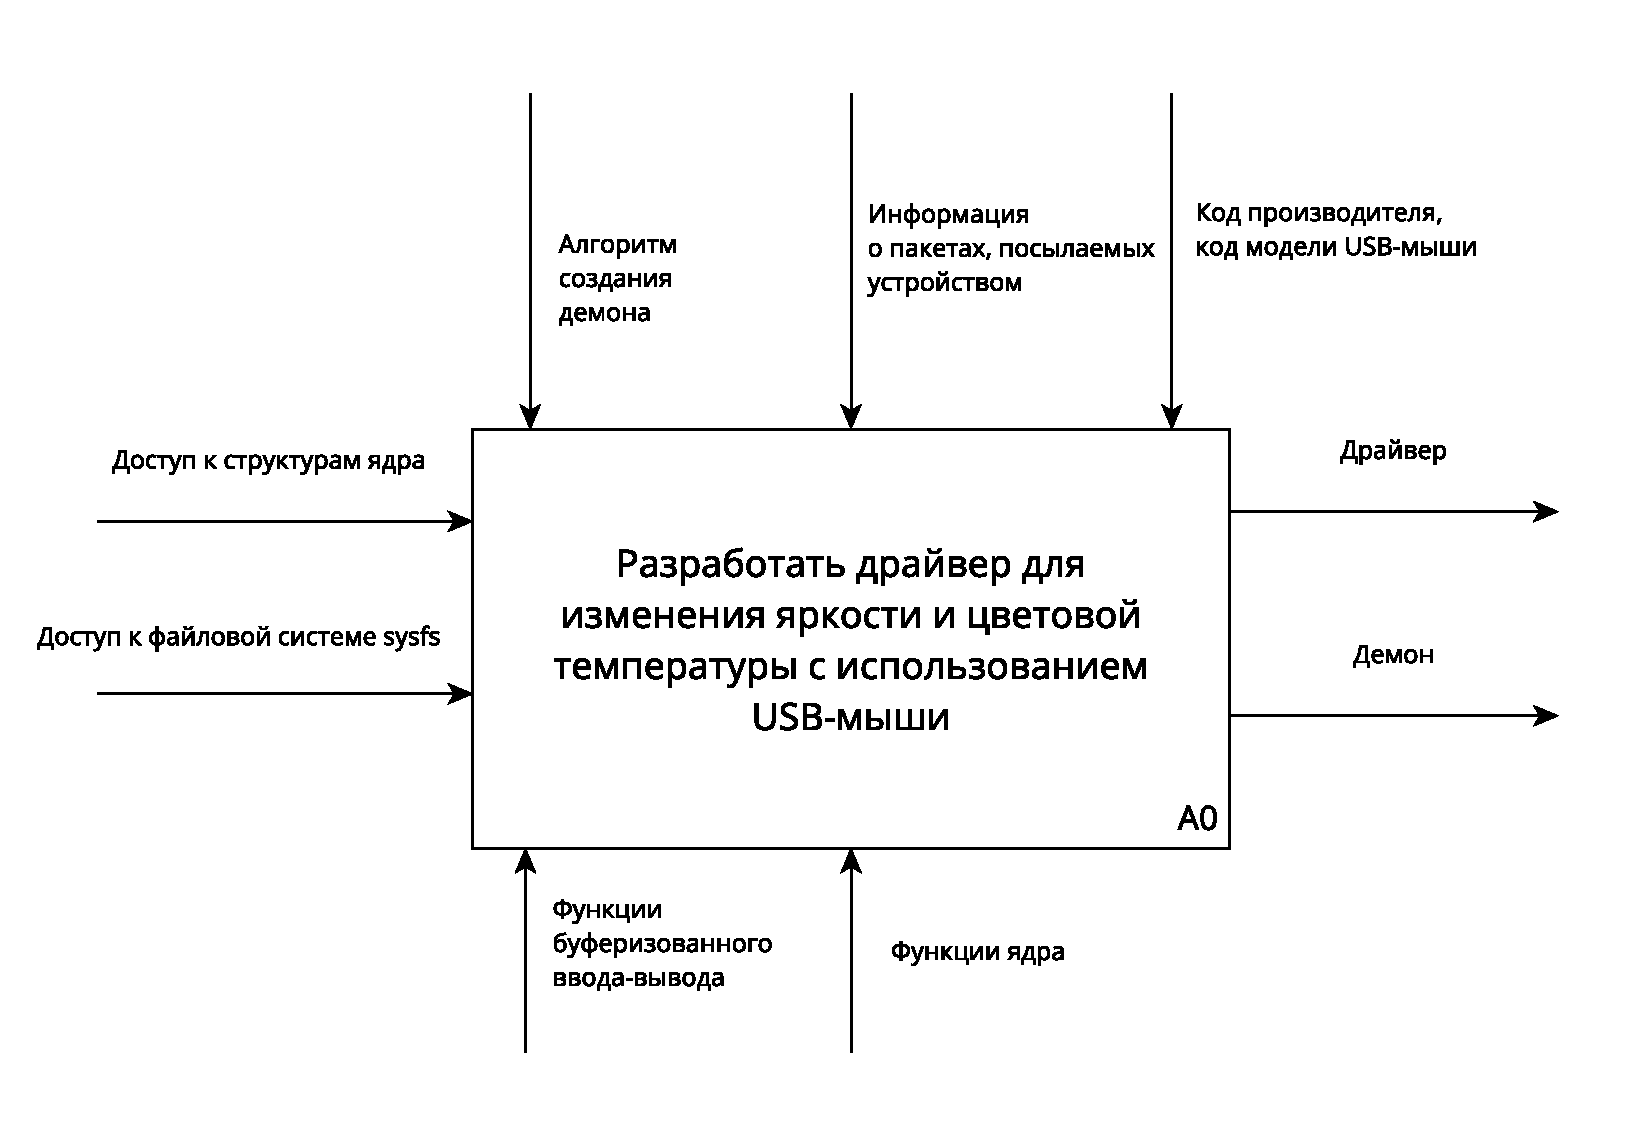
\includegraphics[width=0.9\textwidth]{../img/idef0_0.pdf}
	\caption{Диаграмма IDEF0 нулевого уровня}
	\label{img:idef0_0}
\end{figure}

\begin{figure}[!htb]\centering
	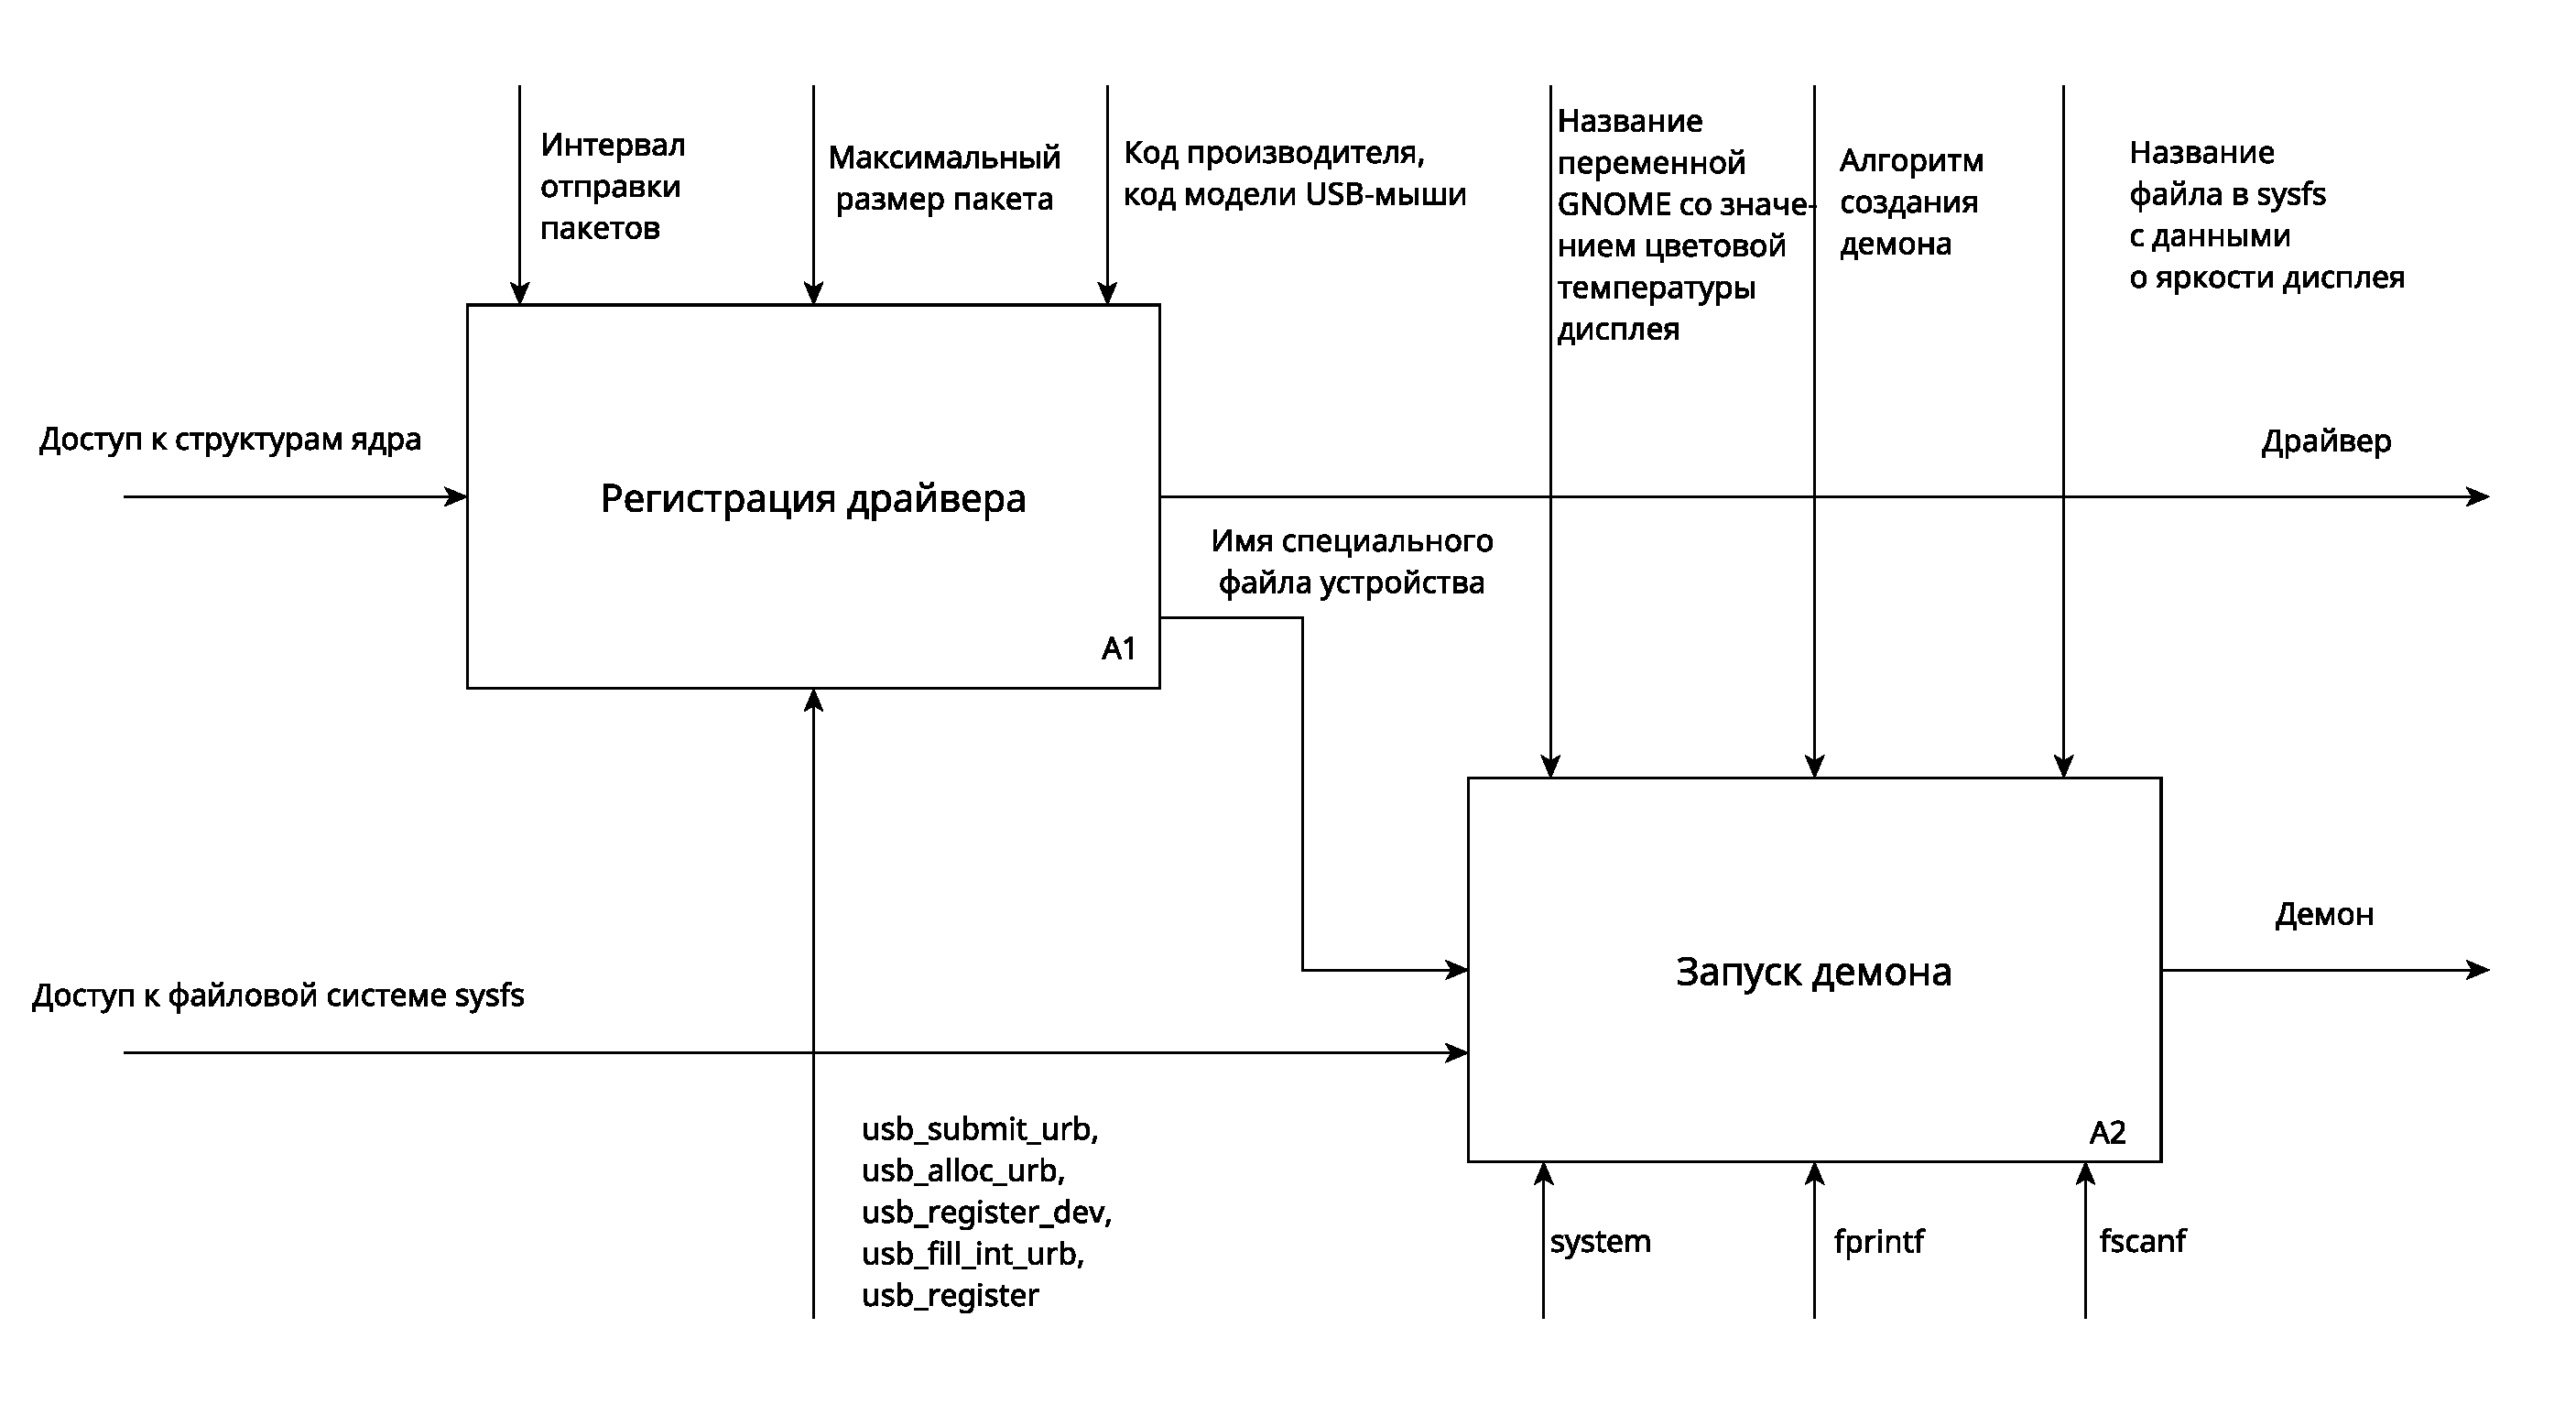
\includegraphics[width=0.9\textwidth]{../img/idef0_1.pdf}
	\caption{Диаграмма IDEF0 первого уровня}
	\label{img:idef0_1}
\end{figure}

\newpage

Структура, содержащая данные для работы драйвера с конкретным USB-устройством, представлена на листинге \ref{lst:usb_aceline}.

\begin{longlisting}
	\caption{Структура usb\_aceline}
	\label{lst:usb_aceline}
	\begin{minted}[frame=single,fontsize = \footnotesize, linenos, xleftmargin = 1.5em]{c}
struct usb_aceline {
  struct usb_device *udev;
  struct usb_interface *interface;
  struct urb *intf_in_urb;
  unsigned char *intf_in_buffer;
  unsigned char *file_buffer;
  size_t intf_in_size;
  size_t time;
  __u8 intf_in_endpoint_addr;
  short connected;
};
	\end{minted}
\end{longlisting}

На рисунке \ref{img:component} представлена диаграмма компонентов.

\begin{figure}[!htb]\centering
	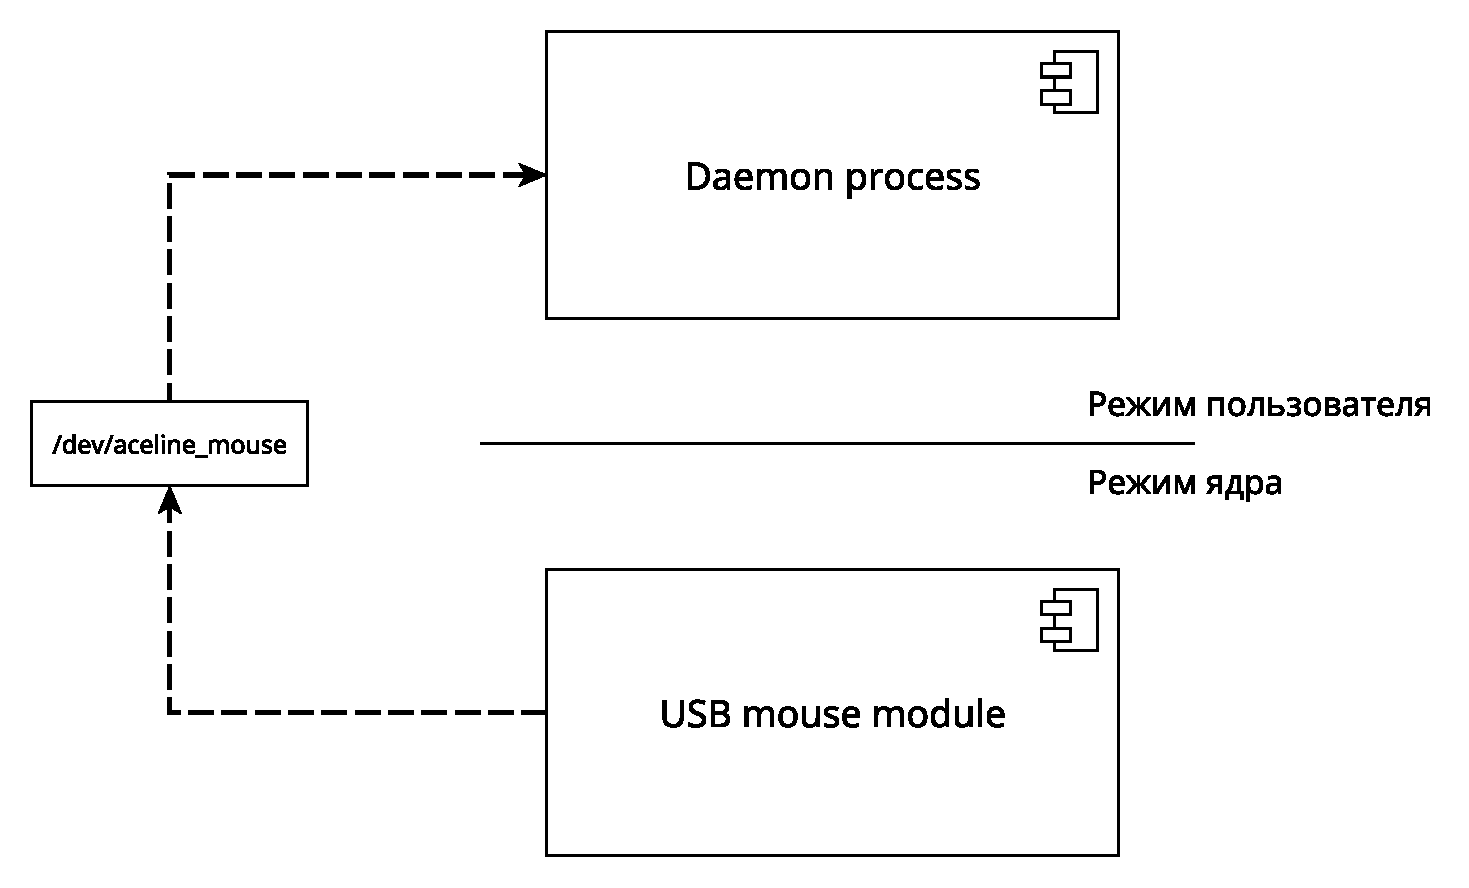
\includegraphics[width=0.9\textwidth]{../img/component.pdf}
	\caption{Диаграмма компонентов}
	\label{img:component}
\end{figure}

На рисунке \ref{img:brightness} представлена схема алгоритма изменения яркости дисплея.

На рисунке \ref{img:night_light_temp} представлена схема алгоритма изменения цветовой температуры дисплея.

На рисунке \ref{img:daemon} представлена схема алгоритма работы демона.

\begin{figure}[!htb]\centering
	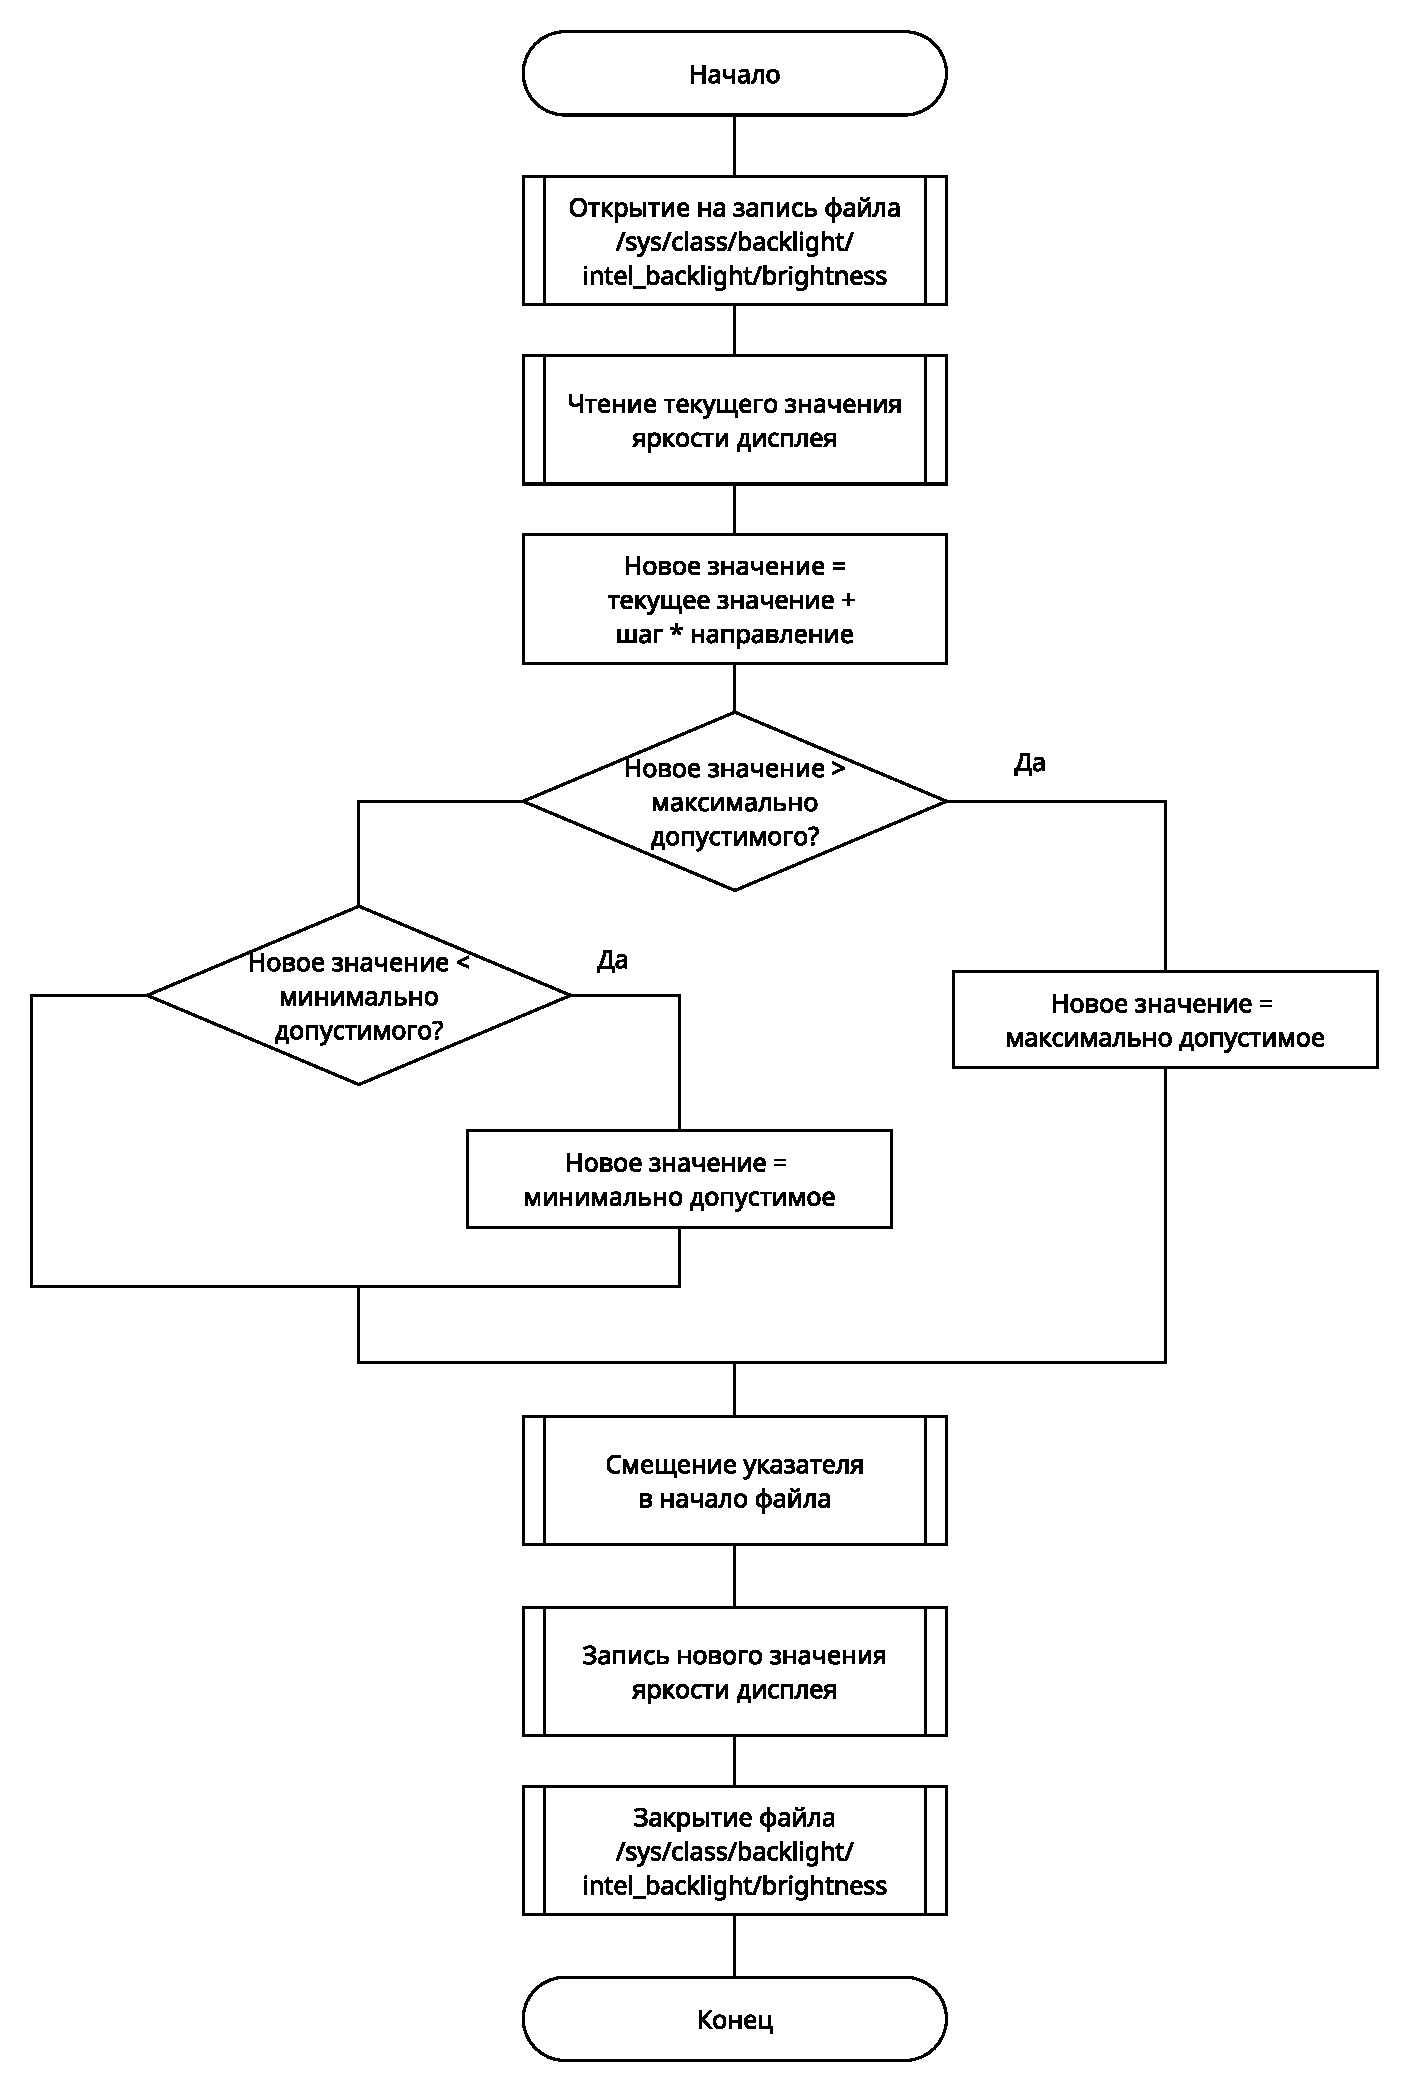
\includegraphics[width=0.9\textwidth]{../img/brightness.pdf}
	\caption{Алгоритм изменения яркости дисплея}
	\label{img:brightness}
\end{figure}

\begin{figure}[!htb]\centering
	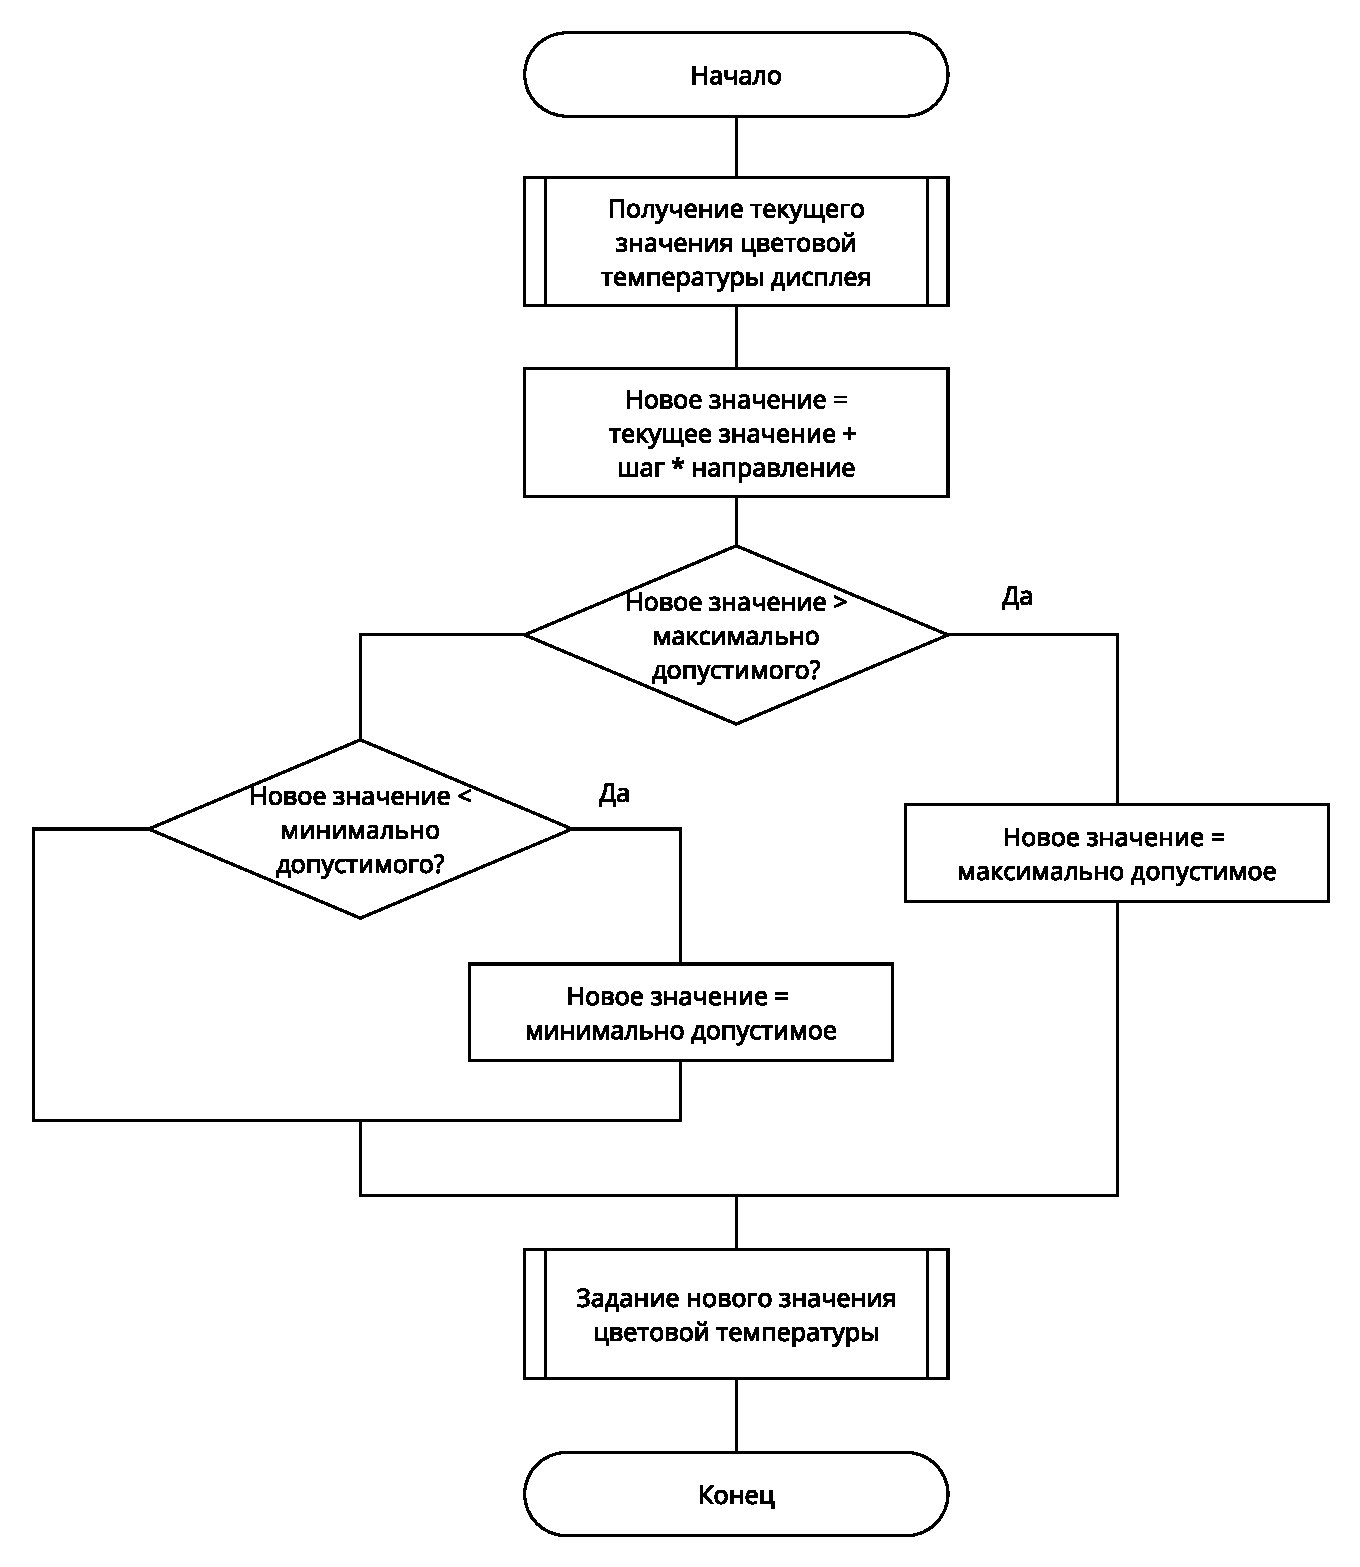
\includegraphics[width=0.9\textwidth]{../img/night_light_temp.pdf}
	\caption{Алгоритм изменения цветовой температуры дисплея}
	\label{img:night_light_temp}
\end{figure}

\begin{figure}[!htb]\centering
	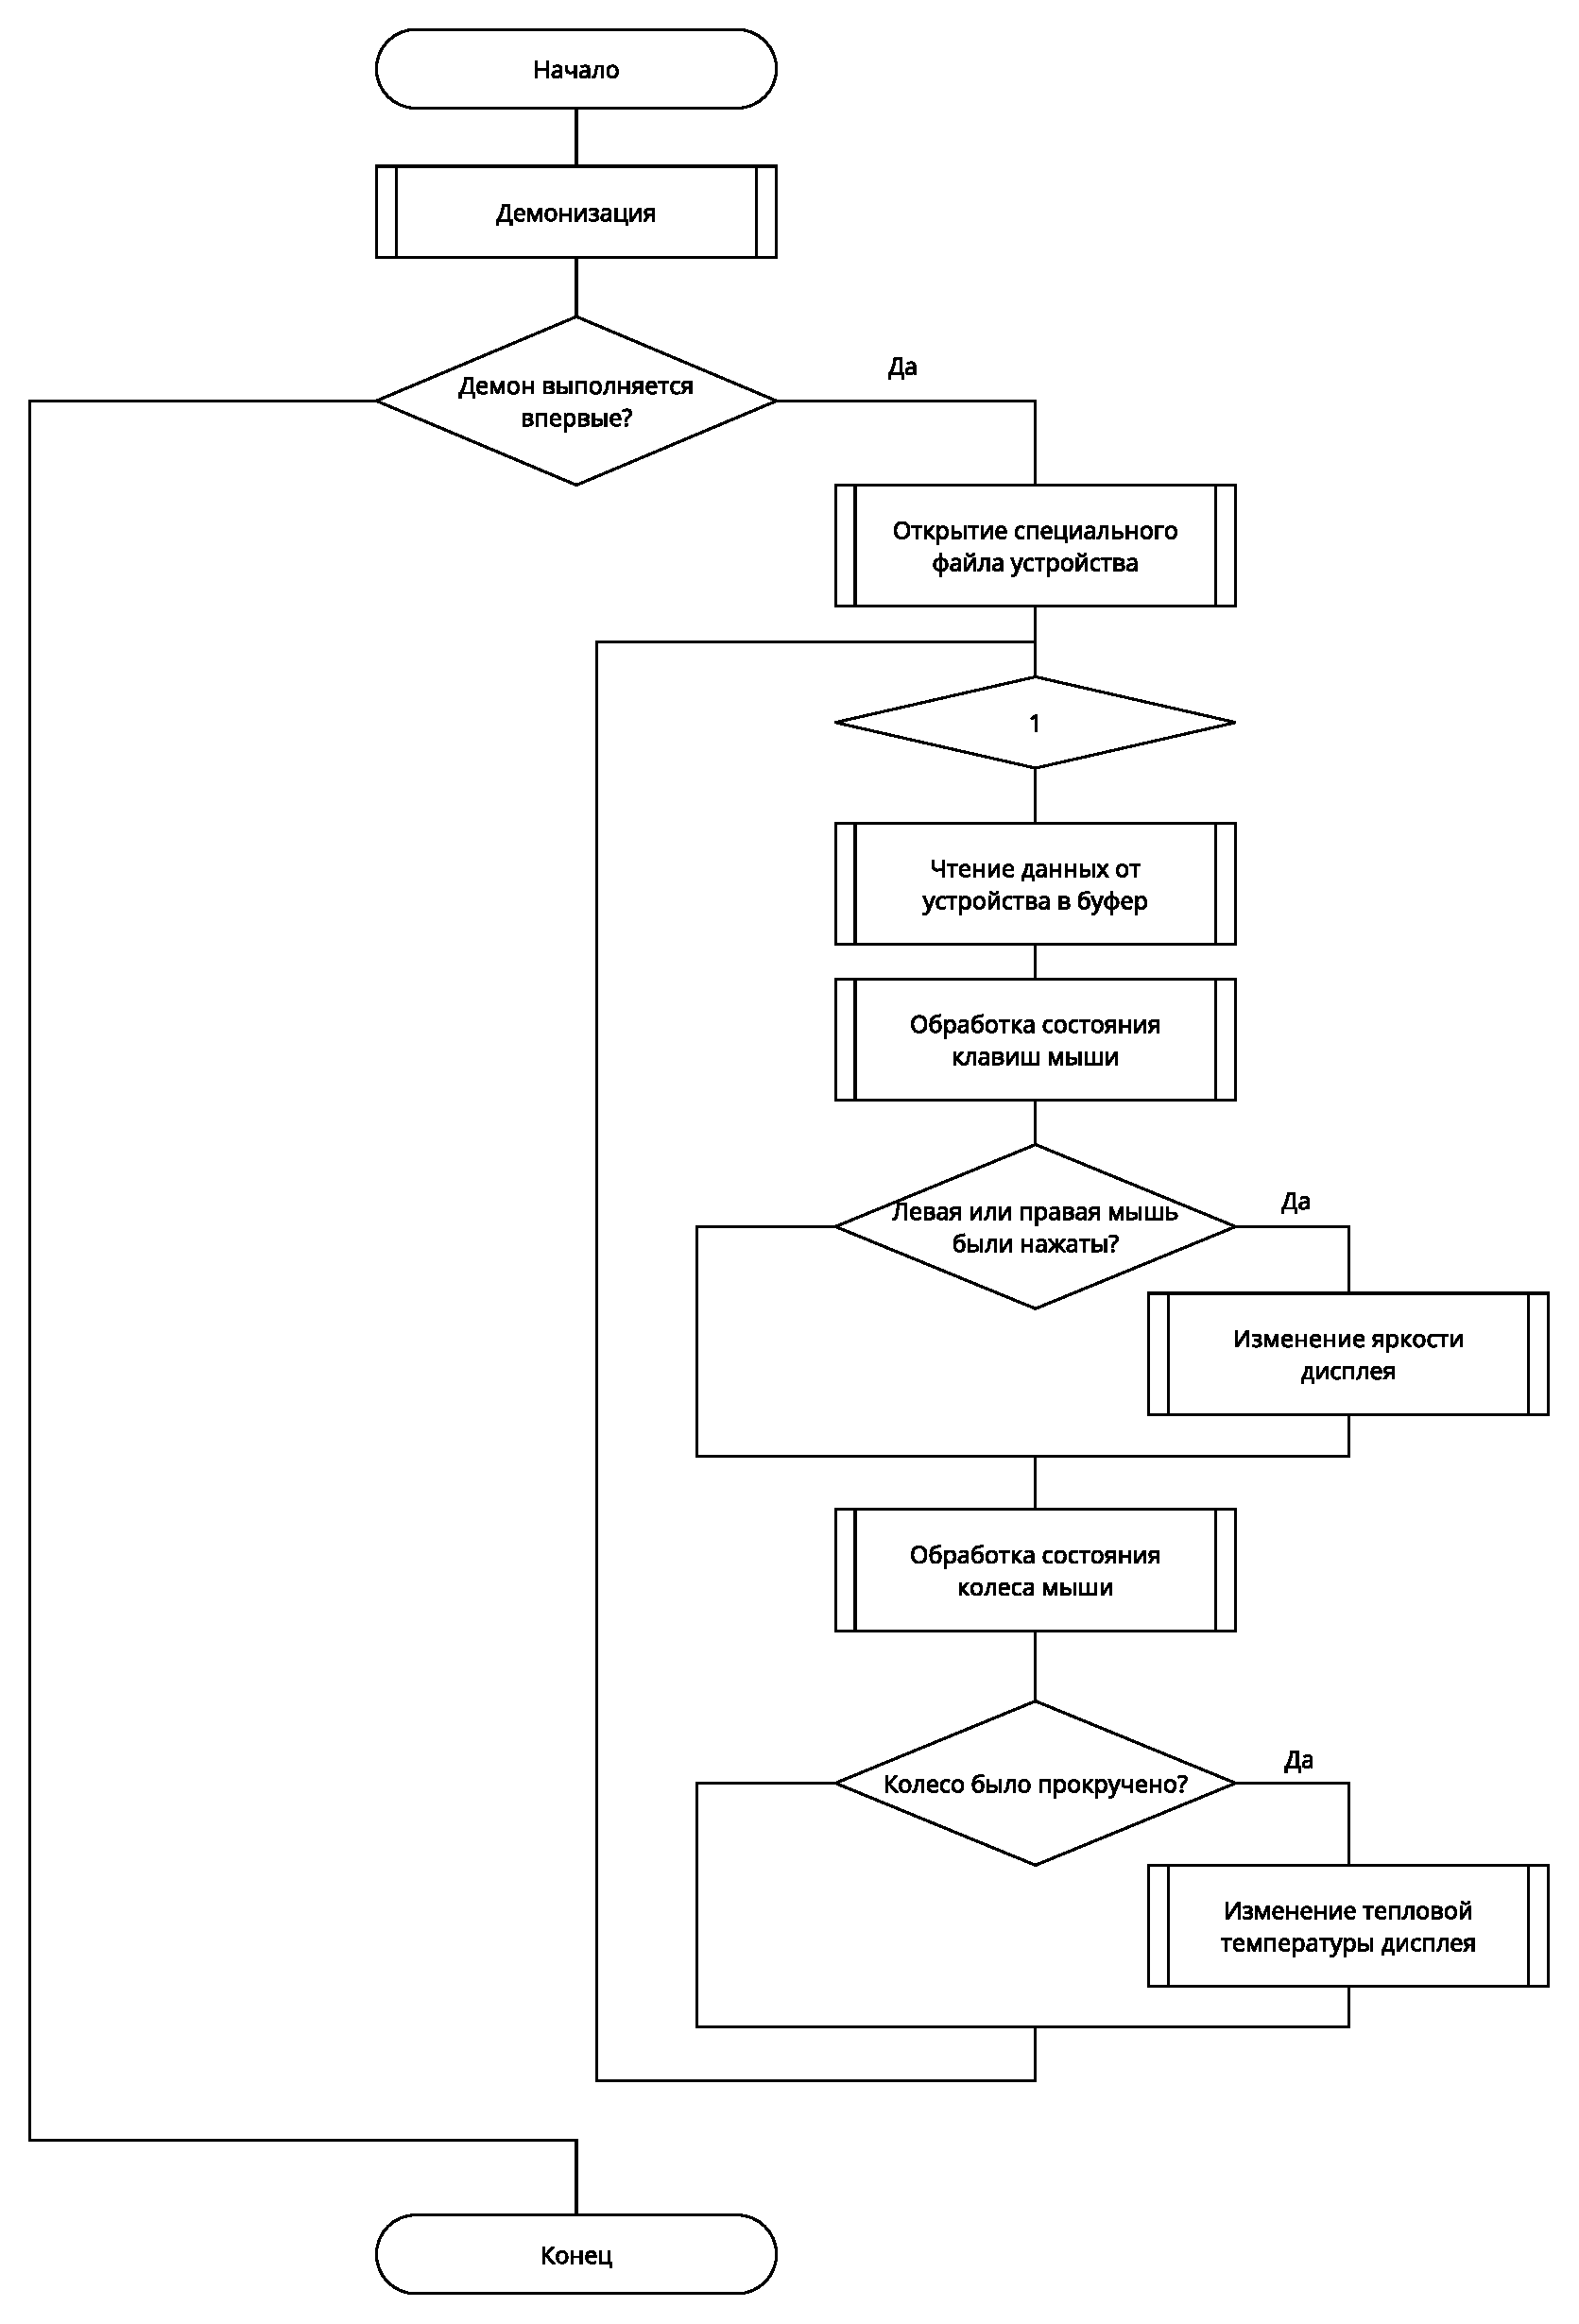
\includegraphics[width=0.9\textwidth]{../img/daemon.pdf}
	\caption{Диаграмма IDEF0 нулевого уровня}
	\label{img:daemon}
\end{figure}
